\documentclass[11pt,spanish]{article}

% Paquetes
\usepackage{amstext}
\usepackage{amssymb}
\usepackage{amsmath}
\usepackage{babel}
    \addto\shorthandsspanish{\spanishdeactivate{~<>}}
    \decimalpoint
\usepackage[style=iso]{datetime2}
\usepackage{fancyhdr}
\usepackage{float}
\usepackage[T1]{fontenc}
\usepackage[a4paper]{geometry}
    \geometry{verbose,tmargin=3cm,bmargin=2cm,lmargin=2.5cm,rmargin=2.5cm}
\usepackage{graphicx}
\usepackage{hyperref}
\usepackage[utf8]{inputenc}
\usepackage{lastpage}
\usepackage{mathptmx}
\usepackage{tasks}
\usepackage{units}
\usepackage{siunitx}

% dibujos 

\usepackage{tikz}
\usepackage{tikz-dimline}
\usetikzlibrary{calc}
% \usetikzlibrary{math}
\usetikzlibrary{arrows.meta}
\usetikzlibrary{snakes}
\usetikzlibrary{decorations}
\usetikzlibrary{decorations.pathmorphing}
\usetikzlibrary{patterns}

% tipo de fuente 
\usepackage{lmodern}

\pagestyle{fancy}
\lfoot{\small DF, FCEyN, UBA}
\cfoot{\tiny Actualizado el {\today} a las {\DTMcurrenttime}}
\rfoot{\small Pág. {\thepage} de \pageref{LastPage}}

\begin{document}

% Título
    \begin{center}
    \textsc{\large Física 2 (Física) -- Cátedra Diego Arbó}
    \par\end{center}{\large \par}
    
    \begin{center}
    \textsc{\large Primer Cuatrimestre de 2025}
    \par\end{center}{\large \par}
    
    \begin{center}
    \textsc{\large Guía 10: Interferencia}
    \par\end{center}{\large \par}

% Comienzo 
\begin{enumerate}


\section*{Condiciones para la interferencia}

% Ejercicio 1

    \item Diga qué entiende por luz cuasi monocromática y dé algunos ejemplos.
    
% Ejercicio 2
    
    \item ¿Bajo qué condiciones se puede decir que dos fuentes son coherentes?
    ¿Es posible observar interferencia de la luz proveniente de dos tubos
    fluorescentes? ¿Por qué? Diga cuándo es posible observar interferencia.

% Ejercicio 3

    \item ¿Es posible observar interferencia entre dos haces de luz
    monocromática de igual frecuencia y linealmente polarizada, si los campos
    eléctricos de ambos haces...
    
    \begin{enumerate}
        \item son perpendiculares?
        \item forman un ángulo de $45^\circ$?
        \item son paralelos?
    \end{enumerate}

% Ejercicio 4
    
    \item ¿Es posible observar interferencia entre dos ondas monocromáticas de
    igual frecuencia si...
    
    \begin{enumerate}
        \item tienen amplitudes muy diferentes?
        \item tienen amplitudes diferentes pero cercanas? (por ejemplo $0.5 < \nicefrac{A_1}{A_2} < 2$)
        \item tienen igual amplitud?
    \end{enumerate}

% Ejercicio 5

    \item Considere dos fuentes sonoras (dos parlantes) que emiten una misma
    señal. Analice la coherencia de ambas fuentes en los siguientes casos.
    
    \begin{enumerate}
        \item La señal es una señal armónica de frecuencia $\omega$.
        
        \item La señal es periódica con período $\tau$ (no necesariamente
        armónica).
        
        \item La señal es ruido blanco\footnote{El ruido blanco es una señal
        aleatoria cuyas muestras cumplen una cierta distribución, por ejemplo
        uniforme o Gaussiana, y además son independientes entre sí.}.
    \end{enumerate}


\section*{División de frente de onda}

% Ejercicio 6

    \item Diga qué entiende por interferómetro por división de frente de onda.
    Mencione los más representativos, haga un esquema de cada uno de ellos
    e indique sus parámetros característicos.

% Ejercicio 7
    
    \item Considere el experimento de dos rendijas de Young.
    \begin{enumerate}
        \item ¿Cuál es el lugar geométrico de los puntos que reciben ondas con
        la misma diferencia de fases?
        
        \item Si la pantalla de observación está lo suficientemente alejada de
        las ranuras, ¿qué aspecto tienen las franjas de interferencia?
    \end{enumerate}
    
% Ejercicio 8

    \item Sea una fuente monocromática ($\lambda=5500$ Å), y un dispositivo
    de Young de las siguientes características: 
    \begin{itemize}
        \item Distancia entre ranuras: $s=3.3$ mm. 
        \item Distancia de las ranuras a la pantalla: $D=3$ m.
    \end{itemize}

    \begin{figure}[H]
        \centering{}
        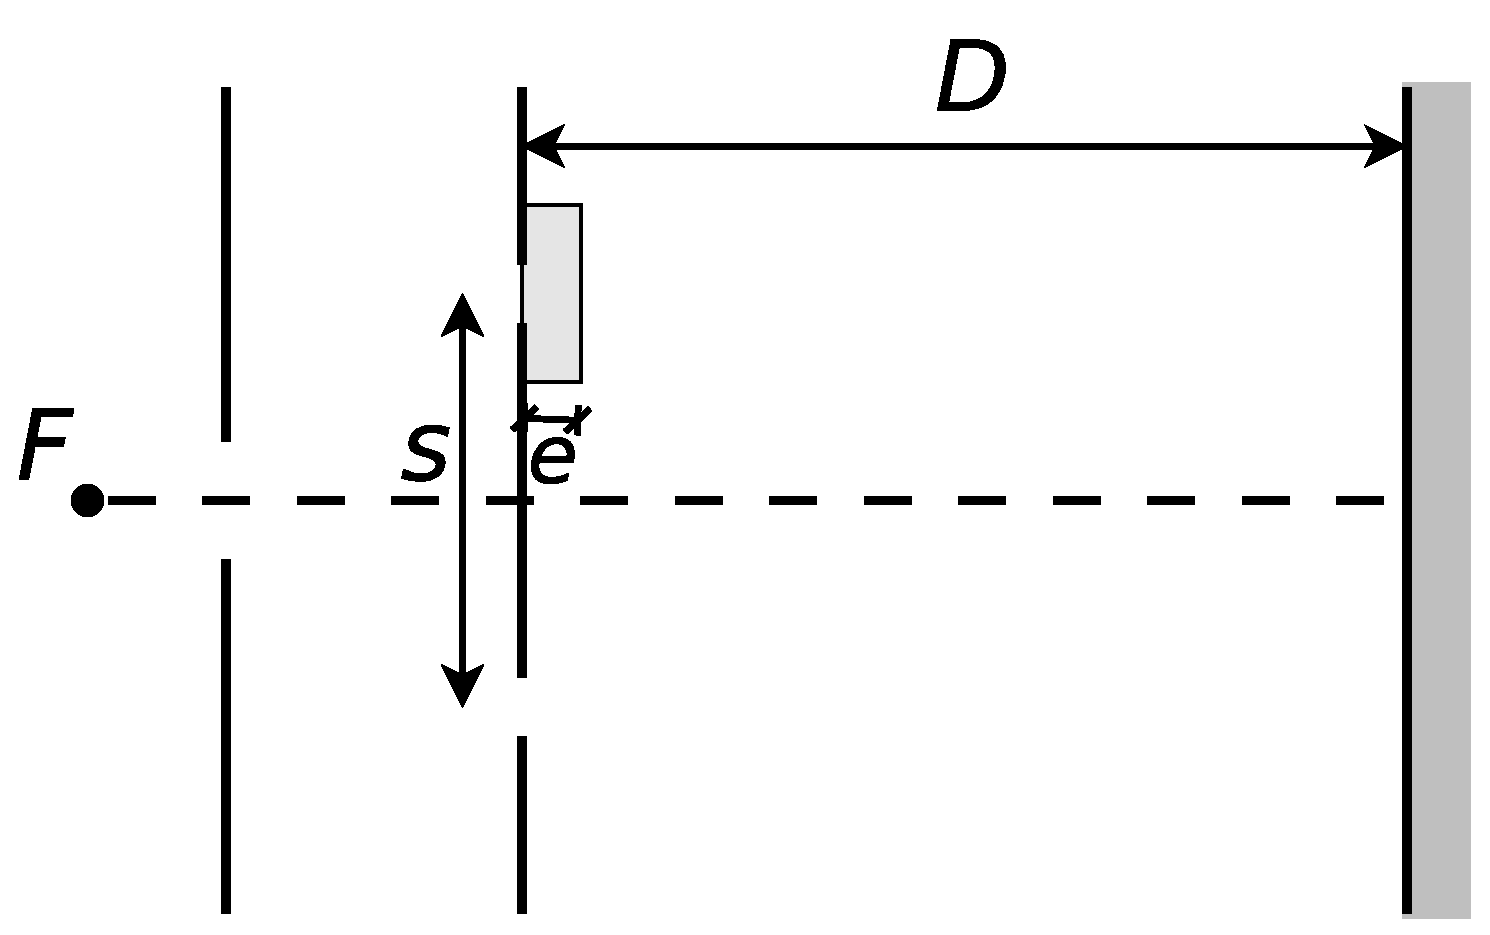
\includegraphics[clip,scale=0.25]{figs/ej5-5}
    \end{figure}
    
    \begin{enumerate}
        \item Calcular la interfranja $i$.
        
        \item Detrás de una de las ranuras se coloca una lámina de vidrio de caras
        paralelas y planas ($e=0.01$ mm) (ver figura). Determinar el sentido
        de desplazamiento de las franjas y la fórmula que da la expresión
        de dicho desplazamiento. Sabiendo que las franjas se han desplazado
        $4.73$ mm, dar el valor del índice de refracción del vidrio. ¿Puede
        detectar dicho corrimiento con una fuente monocromática? ¿Y con una
        policromática?
    \end{enumerate}

% Ejercicio 9
    
    \item ¿Cómo cambia el experimento de Young si la fuente luminosa no está
    simétricamente situada respecto de la ranura, o si, por algún motivo,
    las ondas que llegan a las mismas tienen un cierto desfasaje? ¿Cómo
    puede detectar dicho corrimiento?

% Ejercicio 10

    \item Se tiene el dispositivo para producir interferencia que indica la
    figura. La fuente puntual monocromática de longitud de onda $\lambda$
    (linealmente polarizada en el eje $z$, con amplitud $E_{0}$), ilumina
    dos rendijas separadas por una distancia $a$. La fuente está centrada
    respecto de las rendijas y se encuentra a una distancia $L_{0}$ de
    las mismas. A la izquierda de las rendijas hay dos medios distintos;
    sobre el eje $x$ es $n_{1}$, y debajo del eje $x$ es $n_{2}$ ($n_{2}>n_{1}$);
    a la derecha de las rendijas el índice es $n_{1}$ solamente. A continuación
    de la rendija 2 se coloca una lámina polarizadora cuyo eje de transmisión
    forma un ángulo $\alpha$ con el eje $z$. 
    \begin{description}
        \item [{Datos:}] $a$, $n_{2}$, $n_{1}$, $E_{0}$, $L_{0}$, $L$.
    \end{description}
    
    \begin{figure}[H]
        \centering{}
        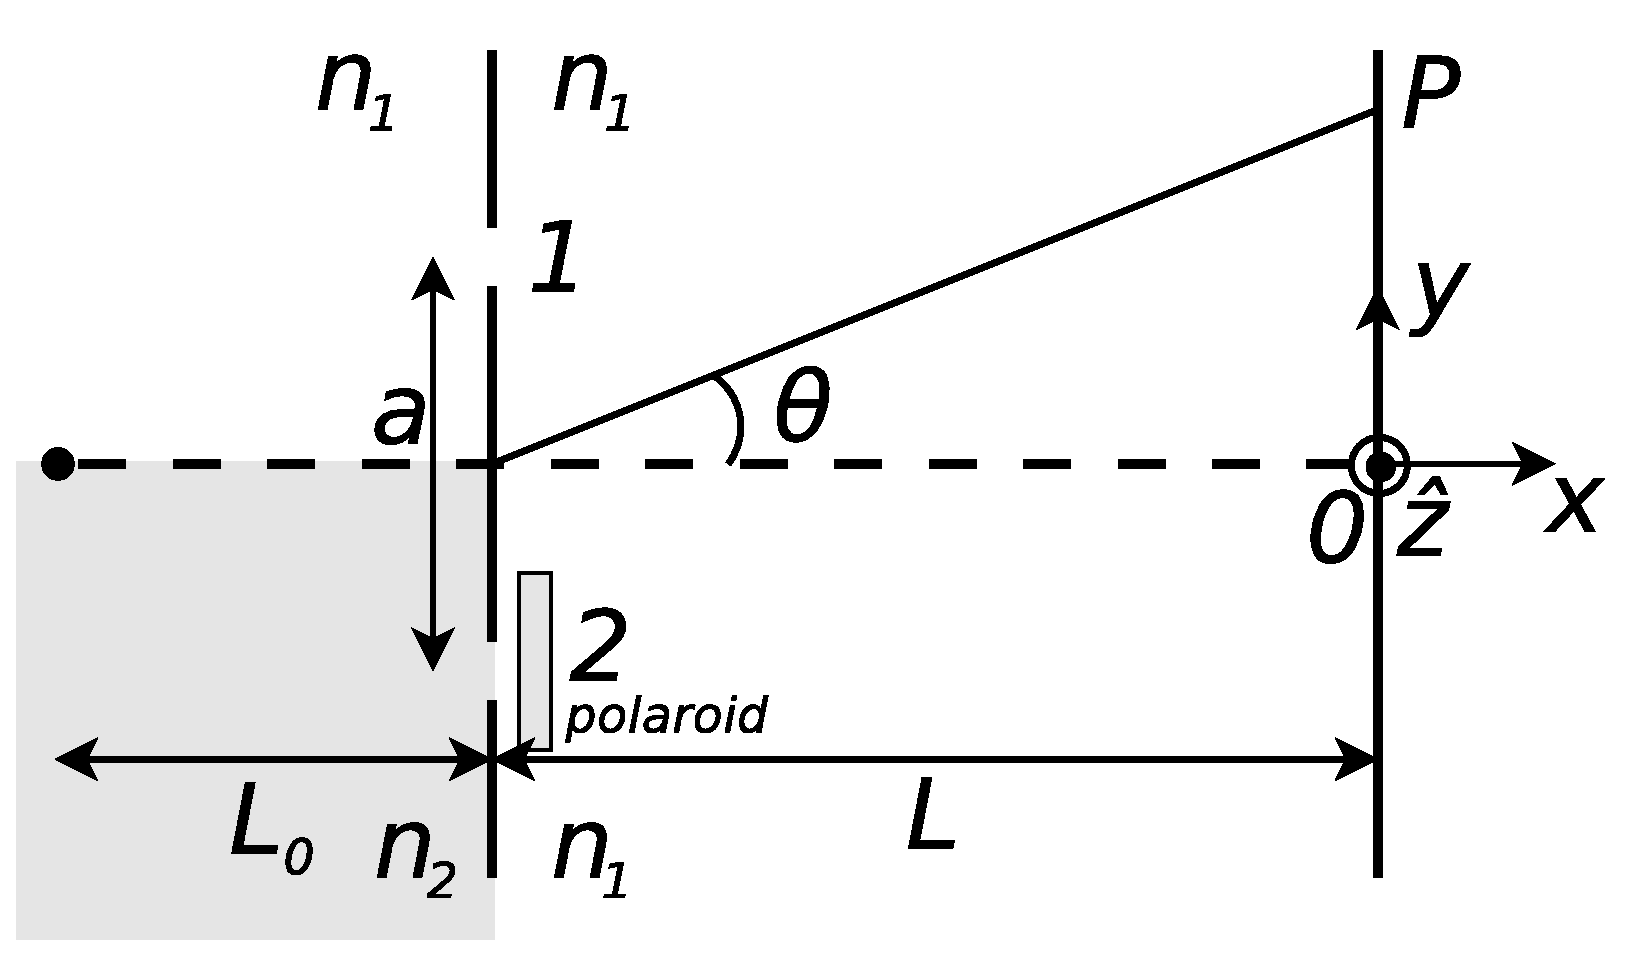
\includegraphics[clip,scale=0.3]{figs/ej5-7}
    \end{figure}

    \begin{enumerate}
        \item ¿Qué efecto produce en el patrón de interferencia la diferencia de
        medios? Explique.
        
        \item Halle el campo eléctrico que sale de la lámina polarizadora como
        función de $\alpha$; expréselo en las coordenadas $y-z$ (sólo el campo
        que sale de la ranura 2; no el total).
        
        \item Halle la expresión de la intensidad en un punto $P$ de la pantalla,
        en función de los campos eléctricos a la salida de las rendijas 1
        y 2. Tenga en cuenta para esto la polarización de dichos campos.
        
        \item Calcule el contraste $c$, definido como:
        $$c=\frac{I_{m\acute{a}x}-I_{m\acute{\imath}n}}{I_{m\acute{a}x}\text{+}I_{m\acute{\imath}n}}$$
        en función del ángulo $\alpha$ y de $\theta$ (ángulo subtendido
        por P). ¿Existen ceros de intensidad para algún $\theta$?
    \end{enumerate}

% Ejercicio 11

    \item Se usa como fuente luminosa para un par de espejos de Fresnel una
    ranura $D$ iluminada con luz monocromática de $4000$ Å y colocada a
    $20$ cm de la intersección de los espejos sobre la bisectriz. Las franjas
    de interferencia observadas a $1$ m de distancia del vértice de los
    espejos tienen una interfranja de $1$ mm. Calcular el ángulo $\alpha$
    entre los planos de los espejos. \textbf{Sugerencia}: nótese que
    la fuente y las dos imágenes son equidistantes de la intersección
    de los espejos. 
    \begin{figure}[H]
        \centering{}
        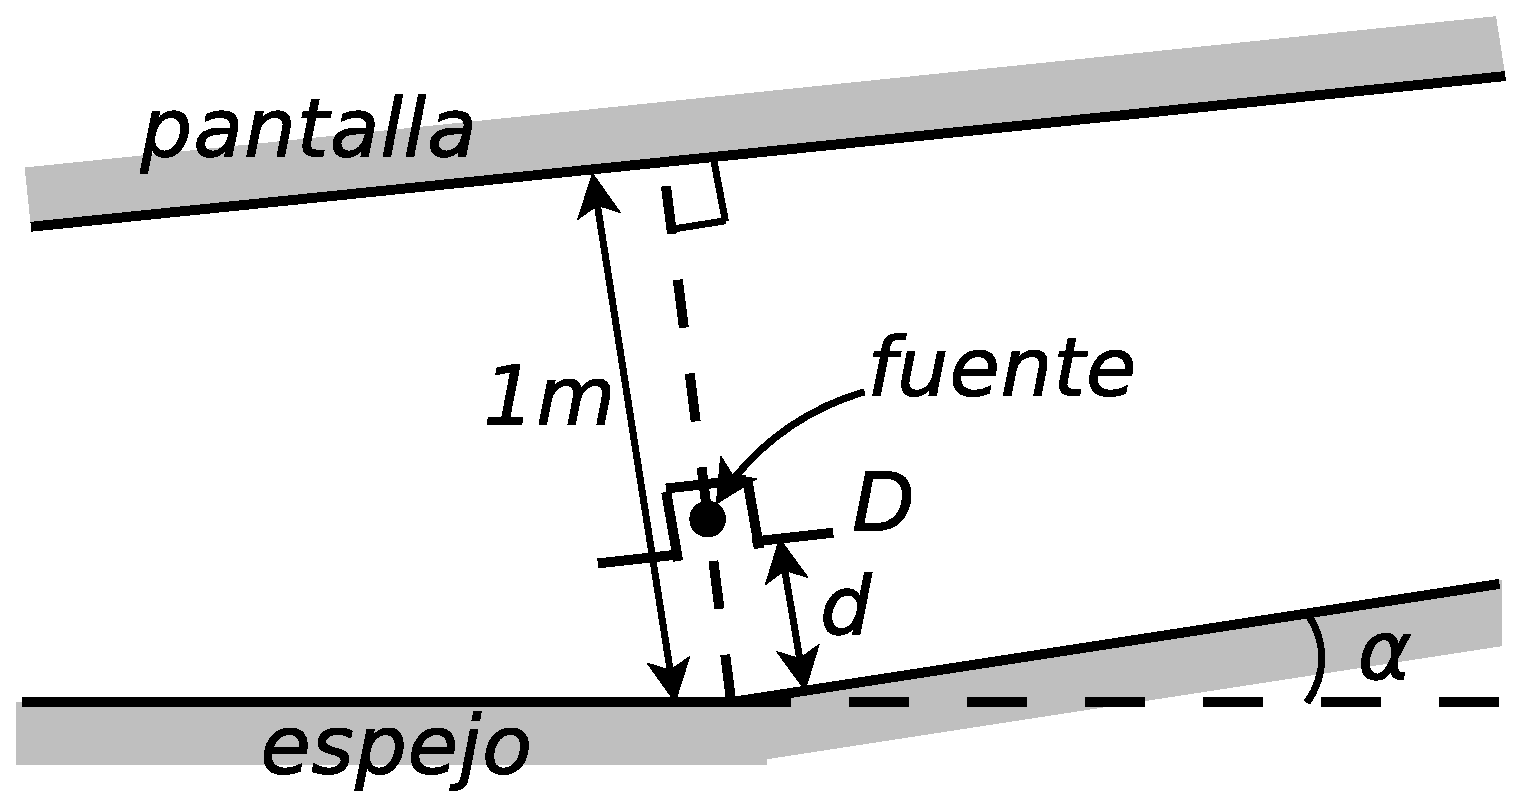
\includegraphics[clip,scale=0.25]{figs/ej5-8}
    \end{figure}
    \begin{description}
        \item [{Datos:}] distancia vértice-pantalla: $1$ m, $d=20$ cm.
    \end{description}

% Ejercicio 12

    \item Examinadas mediante una lupa de distancia focal $f=5$ cm, dos franjas
    de interferencia consecutivas, producidas con los espejos de Fresnel,
    se encuentran a una separación aparente $i'=3$ mm. La distancia entre
    las imágenes de la fuente y la pantalla es $D=4$ m y la separación
    entre las dos imágenes es $d=4$ mm. ¿En qué longitud de onda emite
    la fuente? Nota: suponer que la imagen de las franjas se forma a la
    distancia de visión clara ($d_0=25$ cm) respecto a la lupa.
    
% Ejercicio 13

    \item En un experimento de interferencia con espejos de Fresnel, ¿qué parámetros
    deben modificarse para que la interfranja disminuya? Justifique. Indique
    cómo deben modificarse.

% Ejercicio 14

    \item Considere el siguiente arreglo experimental (llamado biprisma de Fresnel):
    \begin{figure}[H]
        \centering{}
        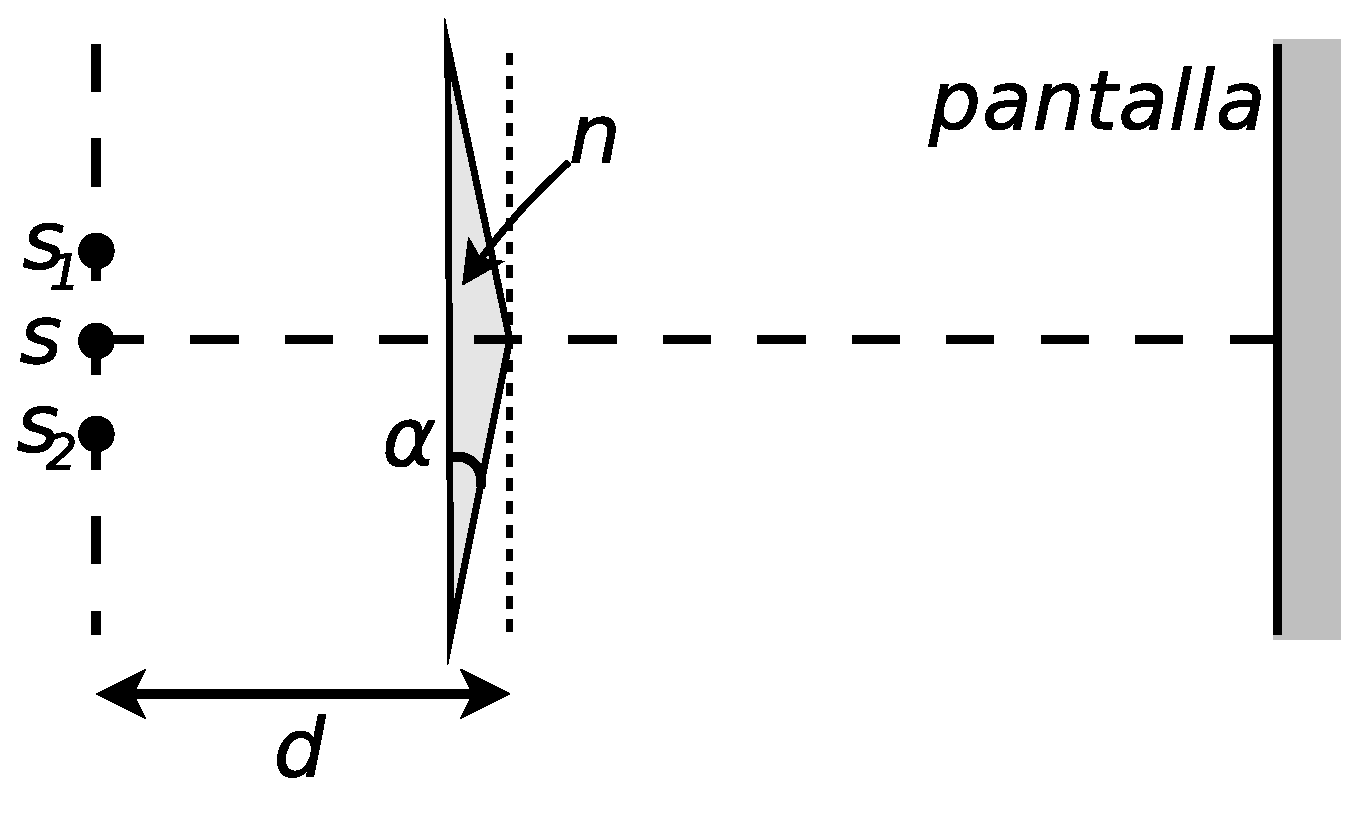
\includegraphics[clip,scale=0.3]{figs/ej5-11}
    \end{figure}
    \begin{enumerate}
        \item Analice cómo se producen las imágenes virtuales en un biprisma de
        Fresnel.
        \item ¿Qué ocurre con la posición de las imágenes si se da vuelta el biprisma,
        es decir, si la arista enfrenta a la pantalla en vez de enfrentar
        a la fuente?
    \end{enumerate}

% Ejercicio 15
    
    \item Un biprisma de Fresnel, hecho de vidrio crown, con ángulo de
    refracción de 1$^{\circ}$ se usa para producir franjas de interferencia.
    La pantalla se ubica a $60$ cm del biprisma y la fuente luminosa a $15$ cm
    de éste. Calcular el ancho de las interfranjas observadas con luz roja
    (línea C de Fraunhofer) y luz azul (línea F de Fraunhofer). 
    \textbf{Observación:} Puede consultar las longitudes de onda y los índices
    de refracción en tablas o en las guías anteriores.
    
% Ejercicio 16

    \item Se observan franjas de interferencia con un biprisma de Fresnel con
    ángulo de $1.5^{\circ}$ e índice de refracción $1.5$. Para esto se usa una
    fuente de luz de $4000$ Å situada a $5$ cm del vértice, y una pantalla
    situada a $1$ m del biprisma. Si, dejando todas las demás condiciones
    iguales, se cambia el biprisma por uno de ángulo $3^\circ$ e índice $1.6$;
    ¿en cuánto varió la interfranja?

% Ejercicio 17
    
    \item En un experimento de interferencia con un biprisma de Fresnel, ¿qué
    parámetros se pueden modificar para que la interfranja aumente?

% Ejercicio 18

    \item Se tiene un dispositivo para producir interferencia consistente en
    una fuente puntual y monocromática $S$, que emite con longitud de
    onda $\lambda$, que se encuentra a una distancia $D_{1}$ de un biprisma
    compuesto por dos prismas delgados de distintos índices y ángulos:
    $n_{1}$, $\alpha_{1}$ ($y>0$) y $n_{2}$, $\alpha_{2}$ ($y<0$).
    El dispositivo se muestra en la figura.
    \begin{figure}[H]
        \centering{}
        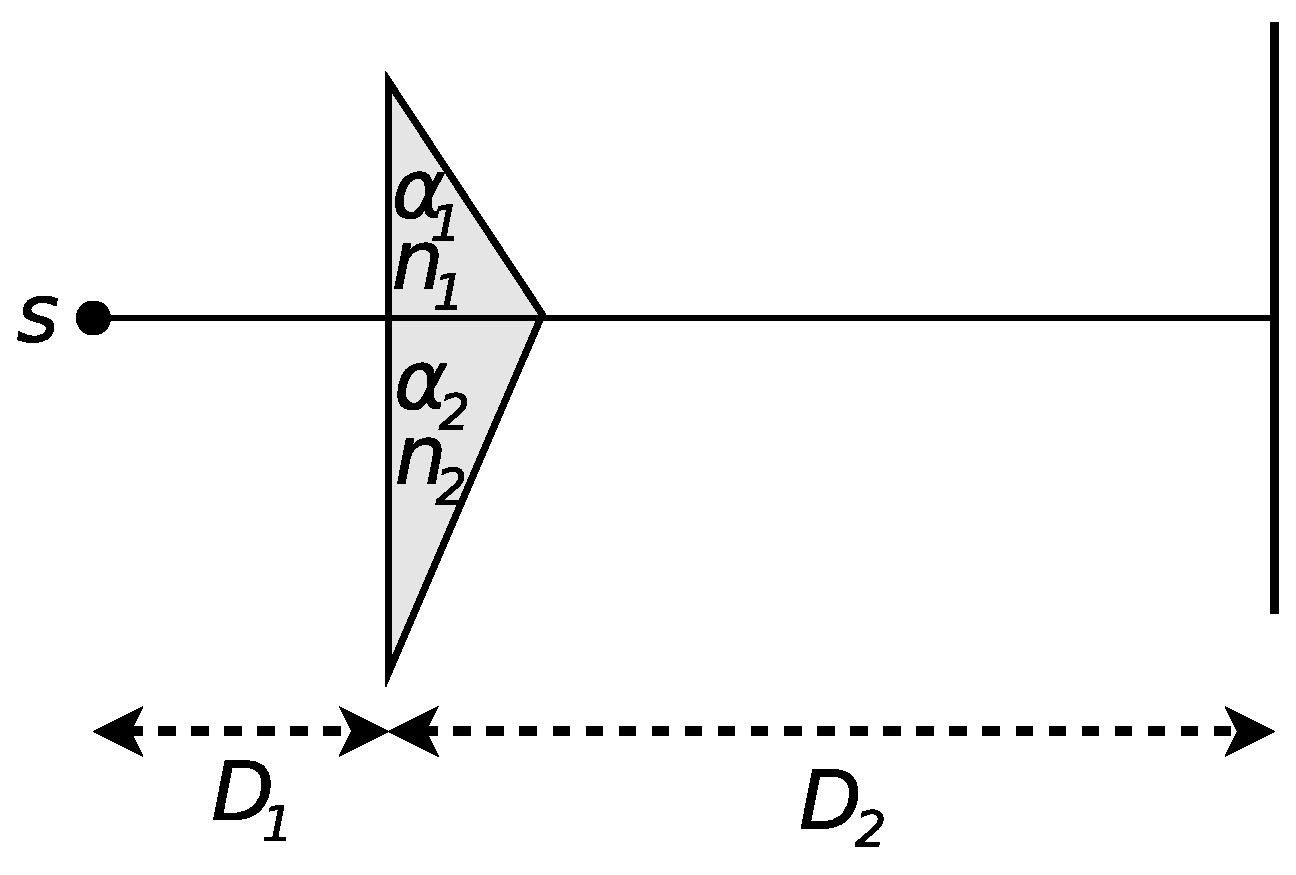
\includegraphics[clip,scale=0.3]{figs/ej5-15}
    \end{figure}

    \begin{enumerate}
        \item Hallar la ubicación de las imágenes $S_{1}$ y $S_{2}$ por la
        refracción en ambas zonas del biprisma, que observaría una persona
        ubicada a la derecha del mismo. 

        \item Marque en una figura la zona donde se produce la interferencia.

        \item Para un punto $P$ genérico sobre la pantalla, calcule el desfasaje
        $\delta$. Sugerencia: piense en los rayos que llegan a $P$ como
        provenientes de las imágenes halladas en (a).

        \item Calcule la interfranja sobre la pantalla. 

        \item Halle la posición de los máximos sobre la pantalla. Si Ud. observara
        este fenómeno sin conocer los parámetros del dispositivo, ¿qué podría
        hacer para distinguir cuál es el orden con $m=0$? 

        \item ¿Cómo debe ser la relación $\alpha_{1}/\alpha_{2}$ para que el máximo
        con $m=0$ esté en la línea determinada por la fuente y el vértice
        del biprisma?
    \end{enumerate}

% Ejercicio 19
    
    \item ¿Por qué motivo se puede concluir, en el experimento del espejo de
    Lloyd, que la luz reflejada ha sufrido un desfasaje de $180^{\circ}$?

% Ejercicio 20

    \item Haga un cuadro comparativo de las magnitudes que caracterizan a los
    distintos interferómetros por división de frente e indique en cada
    uno de ellos cómo se divide el frente. 

    
\section*{División de amplitud}

% Ejercicio 21

    \item Diga qué entiende por interferómetro por división de amplitud. Enumere
    los más representativos e indique en un esquema sus parámetros característicos.
    
% Ejercicio 22

    \item ¿Qué entiende por franjas localizadas de interferencia? ¿En qué casos
    están localizadas las franjas en un interferómetro por división de
    amplitud? Justifique sus respuestas.

% Ejercicio 23

    \item En una lámina de caras paralelas indique la zona del espacio en que
    se observa interferencia para fuente puntual y para fuente extensa.
    En el primer caso calcule la posición de las imágenes de la fuente. 

% Ejercicio 24
    
    \item En la lámina de caras paralelas que se indica en la figura, indique
    qué condición debe cumplirse para que los rayos 1 y 2 interfieran
    constructivamente. Cuando eso sucede, ¿qué pasa con los rayos 3 y
    4? ¿Qué sucede si se usan otras relaciones entre los índices?
    ($n_{1}>n_{2}>n_{3}$).

    \begin{figure}[H]
        \centering{}
        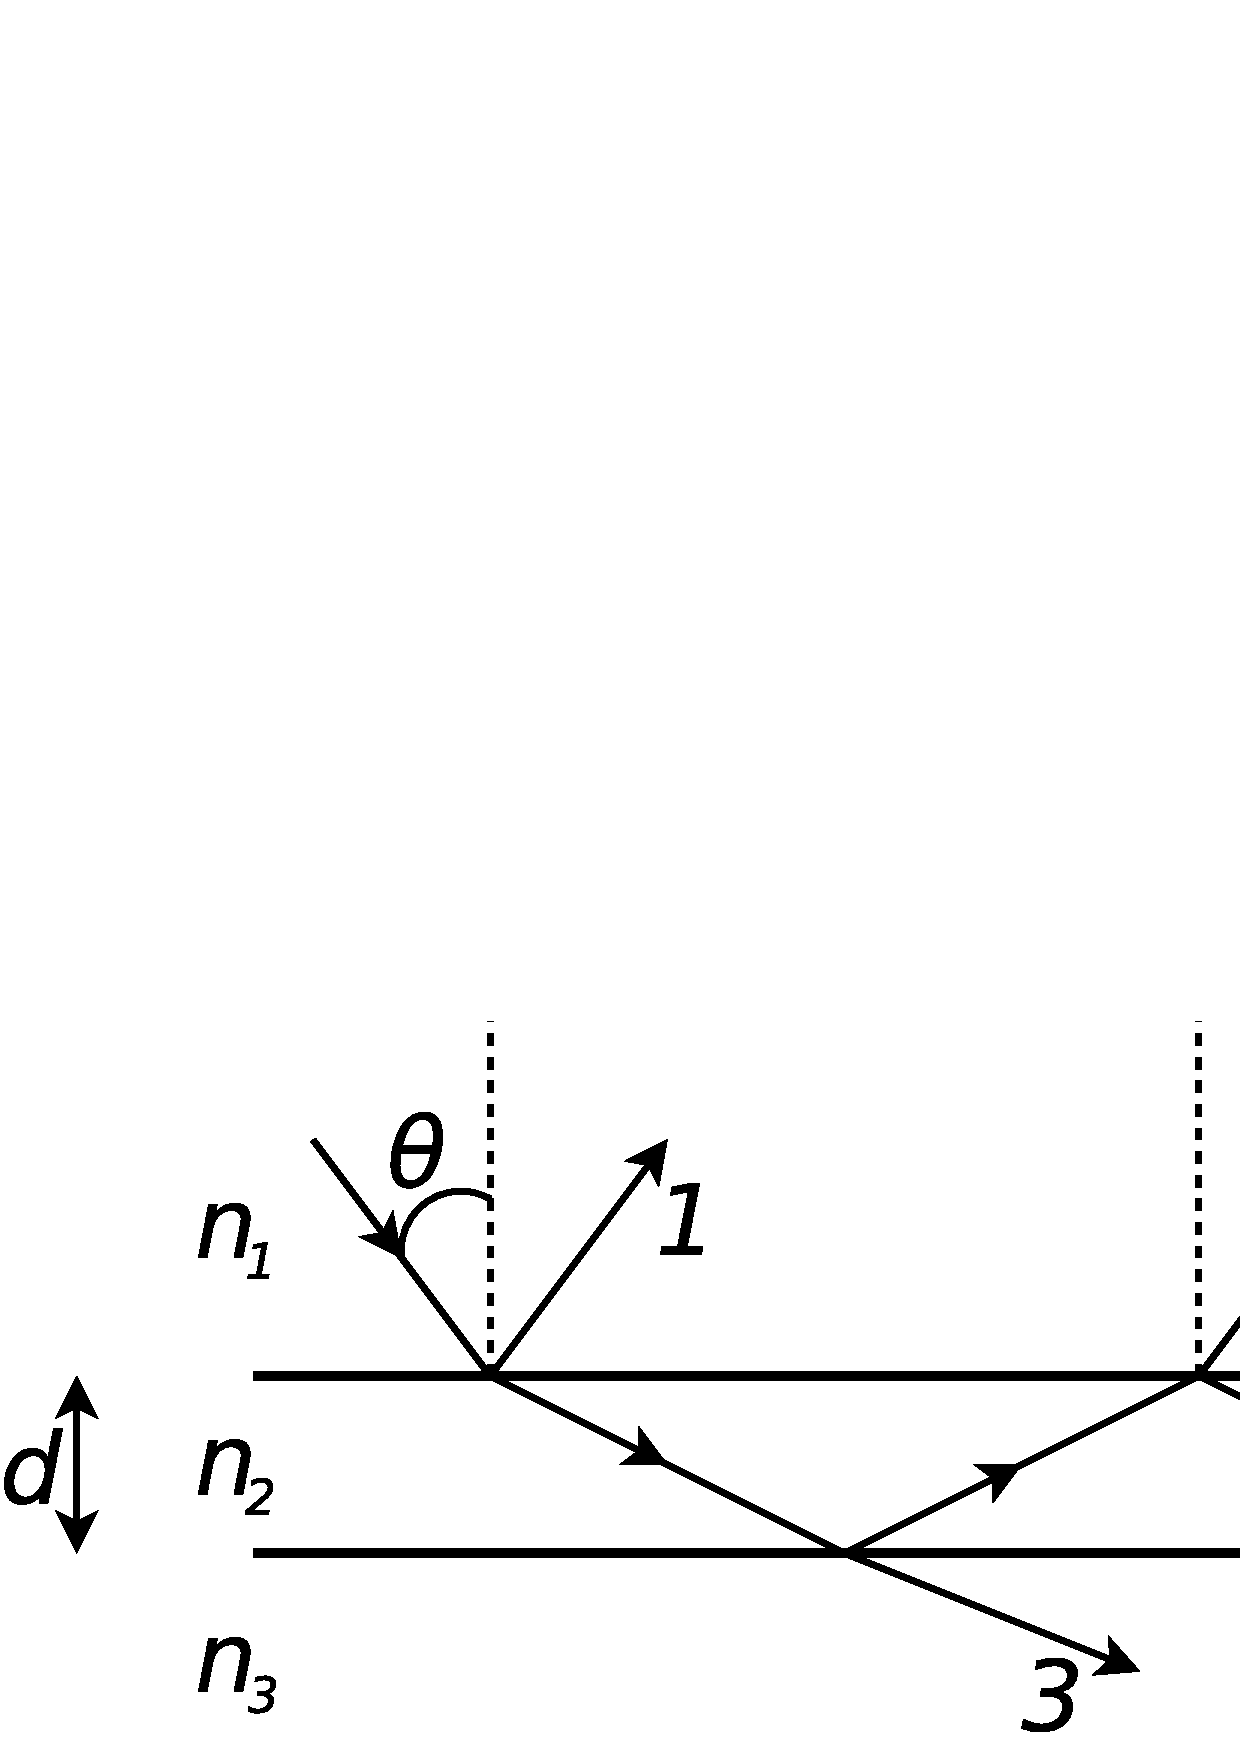
\includegraphics[clip,scale=0.3]{figs/ej5-21}
    \end{figure}

% Ejercicio 25

    \item Una lámina de vidrio de $0.40$ $\mu$m de espesor es iluminada por
    un haz de luz blanca normal a la lámina. El índice de refracción es
    de $1.5$. ¿Qué longitudes de onda dentro de los límites visibles
    del espectro serán intensificadas en el haz reflejado? (espectro visible:
    $40\times10^{-6}\unit{cm}\le\lambda\le79\times10^{-6}\unit{cm}$). 

% Ejercicio 26

    \item ¿Por qué se llaman franjas de igual inclinación a las que aparecen
    en una lámina de caras paralelas iluminada por una fuente extensa?

% Ejercicio 27

    \item Una cuña de aire es iluminada de tal forma que si incide luz de longitud
    de onda $\lambda=$5000 Å normalmente a la cara inferior, produce
    franjas paralelas cuya distancia entre mínimos es 1 mm. Describir
    la cuña. 
    
% Ejercicio 28

    \item Se observan anillos de Newton por reflexión, iluminándose una lente
    plano--convexa con luz de longitud de onda $\lambda=650$ nm. ¿Qué
    radio de curvatura tiene la lente si el segundo anillo oscuro tiene
    $d=2.6$ mm de diámetro? 
    
% Ejercicio 29

    \item Se observan anillos de Newton mediante una lámina de vidrio de índice
    de refracción $n_{3}$, una lente de vidrio con $n_{1}\ne n_{3}$
    y un líquido de $n_{2}$ intermedio entre $n_{1}$ y $n_{3}$ (ver
    figura). 

    \begin{figure}[H]
        \centering{}
        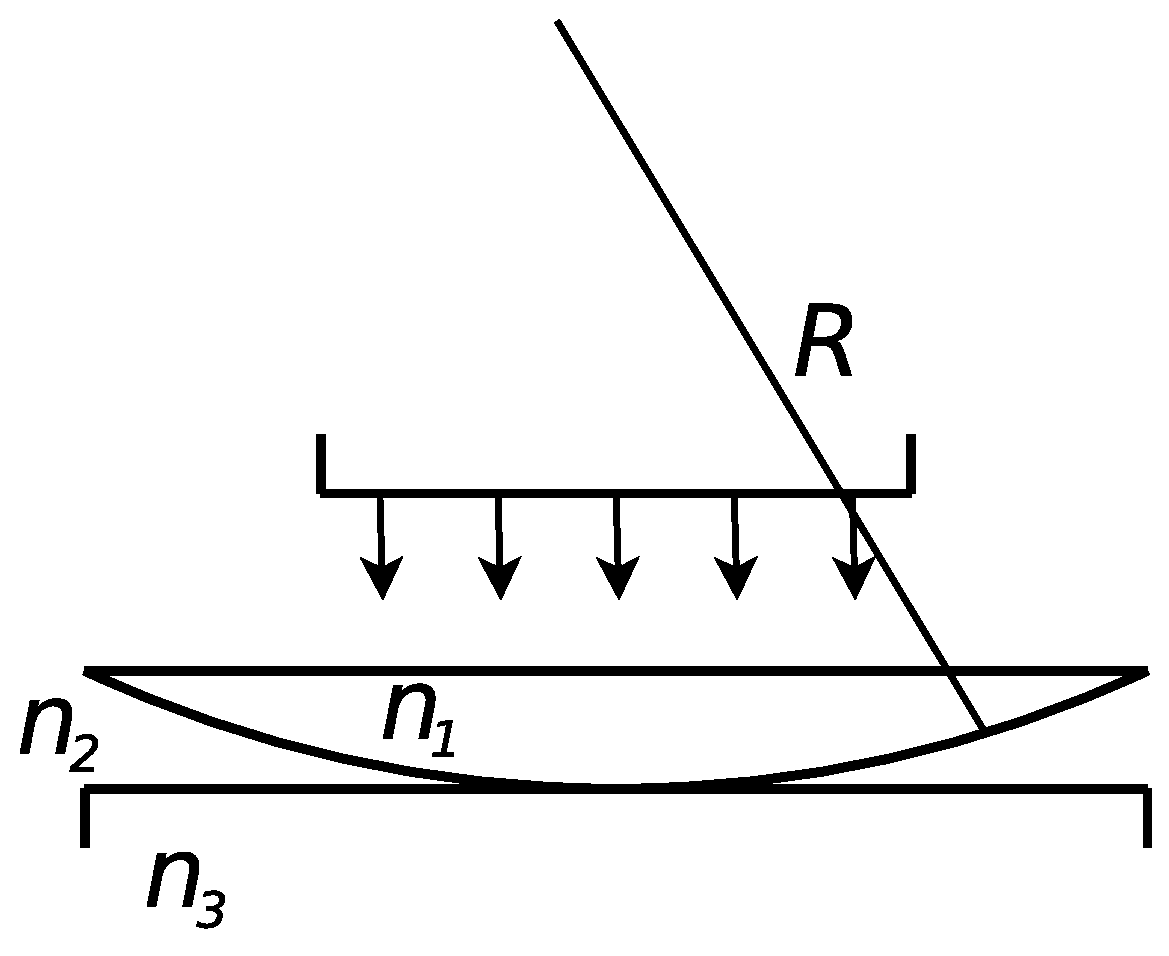
\includegraphics[clip,scale=0.25]{figs/ej5-26}
    \end{figure}

    \begin{enumerate}
        \item ¿Son oscuros o brillantes los centros del sistema de anillos
        observados respectivamente por reflexión y transmisión? 

        \item Suponga ahora que el líquido tiene un índice $n_{2}=1.59$. Si se
        observan los anillos por reflexión siendo $\lambda=5900$ Å, y el
        radio del quinto anillo es de 2 mm, ¿cuál es el radio de curvatura
        de la lente?
    \end{enumerate}
    
% Ejercicio 30

    \item Se observan anillos de Newton con una lente plano--convexa situada
    sobre un vidrio plano, con aire entre medio. ¿Qué pasa con la diferencia
    entre los cuadrados de dos radios consecutivos si: 

    \begin{enumerate}
        \item Se cambia la lente por otra también plano-convexa del mismo radio
        de curvatura, pero de mayor índice de refracción?

        \item Se coloca agua en vez de aire entre la lente y la lámina de vidrio?
    \end{enumerate}
    
% Ejercicio 31

    \item Con el mismo dispositivo de los problemas anteriores se observan anillos
    de Newton por reflexión. ¿Es oscuro o claro el centro de la figura
    de interferencia? ¿Cuál es el radio del tercer anillo brillante? ¿Qué
    sucede con los anillos para un ligerísimo desplazamiento hacia arriba
    de la lente: convergen hacia el centro o se alejan de éste? ¿Por qué?

    \begin{description}
        \item [{Datos:}] $R=1$ m; $d=0.013$ mm; $\lambda=5000$ Å; $n_{1}=1.5$;
        $n_{2}=1.3$; $n_{3}=1.4$.
    \end{description}
 
% Ejercicio 32
   
    \item En un dispositivo para observar anillos de Newton el espacio entre
    la lente y la lámina de vidrio está lleno de líquido. Se observan
    anillos por transmisión. La longitud de onda empleada es $\lambda=5890$
    Å y el radio de curvatura de la lente es de $10$ m. Hallar el índice
    de refracción del líquido sabiendo que el radio del tercer anillo
    brillante es de $3.65$ mm. 

% Ejercicio 33

    \item Considere el dispositivo de anillos de Newton modificado que se muestra
    en la figura. Se observan anillos por reflexión. 

    \begin{figure}[H]
        \centering{}
        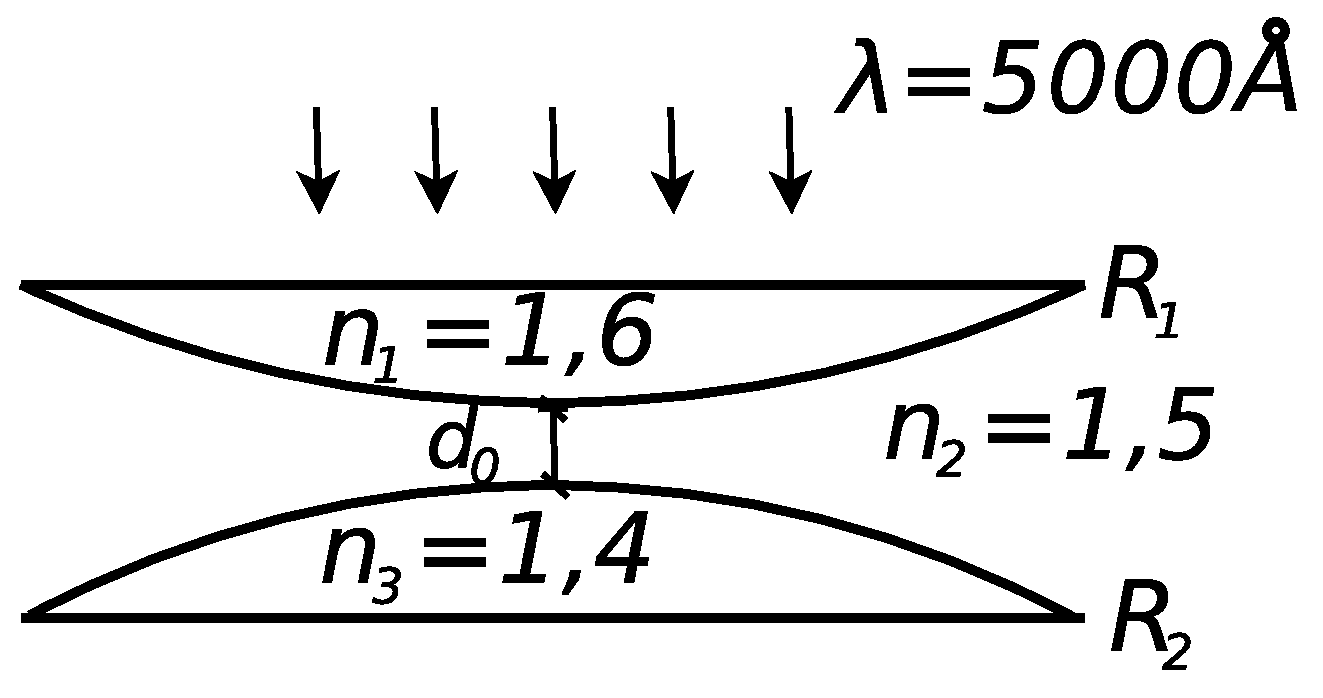
\includegraphics[clip,scale=0.25]{figs/ej5-30}
    \end{figure}

    \begin{enumerate}
        \item ¿Para qué valores de $d_{0}$ el centro de los anillos corresponde
        a un máximo? 

        \item Hallar el mínimo valor de $d_{0}$ para el cual el centro de los anillos
        corresponde a un mínimo. 

        \item Con el valor de $d_{0}$ hallado en (b), calcular la relación que
        debe existir entre los radios de las lentes, $R_{2}(R_{1})$, para
        que el radio del primer anillo oscuro verifique $r_{1}^{2}=10^{15}$
        Å$^{2}$. 
    \end{enumerate}

% Ejercicio 34

    \item Indique en cada uno de los interferómetros por división de amplitud
    estudiados dónde se divide la amplitud. ¿Son iguales las amplitudes
    de los haces que interfieren? En la lámina de caras paralelas compare
    estas amplitudes tanto en la salida por reflexión como por transmisión
    para incidencia normal.

\end{enumerate}

\end{document}
